% Standalone wrapper for the draft chapter. In the thesis, only \input the chapter and
% copy the preamble lines it needs (booktabs, graphicx, xcolor, the two macros below).
\documentclass[11pt,a4paper]{report}
\usepackage[T1]{fontenc}
\usepackage{lmodern}
\usepackage{amsmath}
\usepackage{booktabs}
\usepackage{graphicx}
\usepackage{xcolor}
\usepackage{caption}
\usepackage[margin=2.5cm]{geometry}
\usepackage{hyperref}

\graphicspath{{figures/}}

% Draft markers: \draftnote{...} for notes to the author, \src{KEY} for the source of a
% number (keys in PROVENANCE.md). Redefine both as empty for the final thesis.
\newcommand{\draftnote}[1]{\textcolor{red!70!black}{\footnotesize\textsf{[#1]}}}
\newcommand{\src}[1]{\textcolor{gray}{\footnotesize\textsf{[#1]}}}

\begin{document}
% Draft chapter: computational cost of the particle refinement.
% Numbers from the stage 1 measurements (2026-11-25/26). They are preliminary: the final
% numbers come from one frozen commit (benchmarks/PLAN.md, "Stage 2"). Sources of all
% numbers: PROVENANCE.md (keys in \src{...}). Figures and two tables are generated by
% make_figures.py from the result files.

\chapter{Computational cost of the particle refinement}
\label{ch:performance}

\draftnote{Stage 1 data from several commits (b8a4e7f, 92fef57, 92fef57 with the
uncommitted load balancing). Every number in this chapter will be replaced by the stage 2
measurements on the frozen commit. The structure and the qualitative findings are
expected to remain.}

Refinement reduces the number of particles, but each particle becomes more expensive.
This chapter measures where a refined simulation spends its time. Two kinds of cost
are distinguished:
\begin{itemize}
  \item the \emph{direct} cost of the refinement call itself: the refinement criteria,
        splitting, merging and the shifting of the new particles, and
  \item the \emph{indirect} cost: the right-hand side (RHS) and the other per-step work
        become more expensive per particle when the smoothing length varies in space.
\end{itemize}
Uniform simulations at the coarsest and the finest spacing serve as references. The goal is
to explain the cost of the refinement, not to optimize the implementation. Whether the
refinement pays off, i.e.\ whether it reaches a given error in less wall time than a
uniform simulation, is a question of accuracy and cost together. It is treated with the
vortex street experiment in Chapter~\ref{ch:vortex-street}
\draftnote{label of the E3 chapter}.

% ==========================================================================================
\section{Setup and measurement method}
\label{sec:performance-method}

\paragraph{Test case.}
All measurements use the flow past a cylinder (vortex street) at $\mathrm{Re} = 200$,
because it is the case where refinement is meant to pay off: fine particles are needed
only near the cylinder and in the wake. The setup is summarized in
Table~\ref{tab:performance-setup}. The coarsest spacing gives $D/\Delta x = 7$, which
is too coarse for accurate force coefficients but sufficient to measure the cost. With a
spacing ratio of~2 the finest particles have $D/\Delta x = 14$, with a ratio of~4,
$D/\Delta x = 28$. The cylinder is always discretized with the finest spacing.

\begin{table}[htb]
  \centering
  \caption{Setup of the performance measurements. \src{setups.jl, example
  vortex\_street\_2d\_refinement.jl}}
  \label{tab:performance-setup}
  \small
  \begin{tabular}{lp{0.62\textwidth}}
    \toprule
    domain, cylinder & $20D \times 10D$, $D = 0.1$, cylinder at $5D$ downstream \\
    flow & $U = 1$, $\mathrm{Re} = 200$, inflow and outflow as open boundaries
           (method of characteristics) \\
    fluid model & EDAC, summation density, Wendland C2 kernel, $h = 1.5\,\Delta x$ \\
    spacings & $\Delta x_{\max} = 1/70$; $\Delta x_{\min} = \Delta x_{\max}/2$ or
               $\Delta x_{\max}/4$ \\
    refinement & spatial and vorticity criterion, called every 10 time steps \\
    shifting after refinement & $\theta = 1$, at most 20 iterations \\
    time integration & RDPK3SpFSAL35, $\mathrm{abstol} = 10^{-5}$,
                       $\mathrm{reltol} = 10^{-3}$ \\
    \midrule
    hardware & AMD Ryzen Threadripper 3990X (64 cores), 8 threads on otherwise idle cores \\
    software & Julia 1.13.4, TrixiParticles.jl \draftnote{commit},
               PointNeighbors.jl 4842a89 \\
    \bottomrule
  \end{tabular}
\end{table}

\paragraph{States.}
The cost depends on the state of the flow, since the vorticity criterion refines the wake
as it develops. Two states are measured. The \emph{early} state directly follows the
startup, when only the surroundings of the cylinder are refined. The \emph{developed}
state is taken at $t = 4$: the number of fluid particles at ratio~2 rises from about
10\,600 after the startup to a peak of 15\,700 at $t = 2.9$ and then stays between
14\,600 and 15\,250 up to $t = 8$ \src{P1}. Since a refined simulation cannot be restarted
from a file, the developed state is simulated in the same process before the measurement.

\paragraph{Measured quantities.}
Each measurement runs 100 time steps from the given state and records the wall time of the
parts of a step with timers inside the code. The reported value is the median of three
runs (five for the developed uniform runs). Runs during which other processes slowed
down the threads were discarded. Such stalls occurred even on an otherwise idle machine and
are detected from the time of a trivial per-particle loop.

The times are normalized per step and per fluid particle. Per step, because the refined
simulation takes about the same time step as the uniform fine one (about 950 steps per
unit of simulated time, compared to 470 for the uniform coarse one), so the cost per step is
also the cost per simulated time. Per fluid particle, because the refined and the
uniform simulations have different numbers of particles.

\paragraph{Comparisons.}
Differences of a few percent between separate sessions are common on the shared machine.
Every comparison of two code versions or settings that is reported here therefore runs the
variants in separate processes, alternating in blocks, and includes a repetition of the
reference variant (A/A comparison) as an estimate of the noise.

\paragraph{Neighborhood search.}
With refinement, each fluid particle has its own smoothing length. Two neighborhood searches
are compared:
\begin{itemize}
  \item the \emph{grid} search with one cell size and one search radius, the largest
        compact support in the domain, and
  \item the \emph{tree} search with one radius per particle, $r_a =
        \min(\operatorname{supp}(h_a), R)$, where $R$ is the largest radius. With
        \emph{pruning}, the tree skips leaves that are too far away for the query.
\end{itemize}
Both return the same interacting pairs; this was checked for all pairs of the
Taylor--Green vortex and the pipe flow (Chapter~\ref{ch:implementation}
\draftnote{label}). The tree is under active development, while the grid search is
mature. The comparison here therefore only asks which setup is fastest with refinement; it
is not a benchmark of the two searches.

% ==========================================================================================
\section{Where the time goes}
\label{sec:performance-budget}

Figure~\ref{fig:performance-budget} shows the time per step and fluid particle, split into
the RHS evaluations, the refinement call, the update callback (the update of systems and
neighborhood searches after each step and the particle shifting technique) and the time
integration. Table~\ref{tab:performance-shares} gives the shares of all timed parts for
the refined runs, and Table~\ref{tab:performance-uniform} the absolute times.

\begin{figure}[htb]
  \centering
  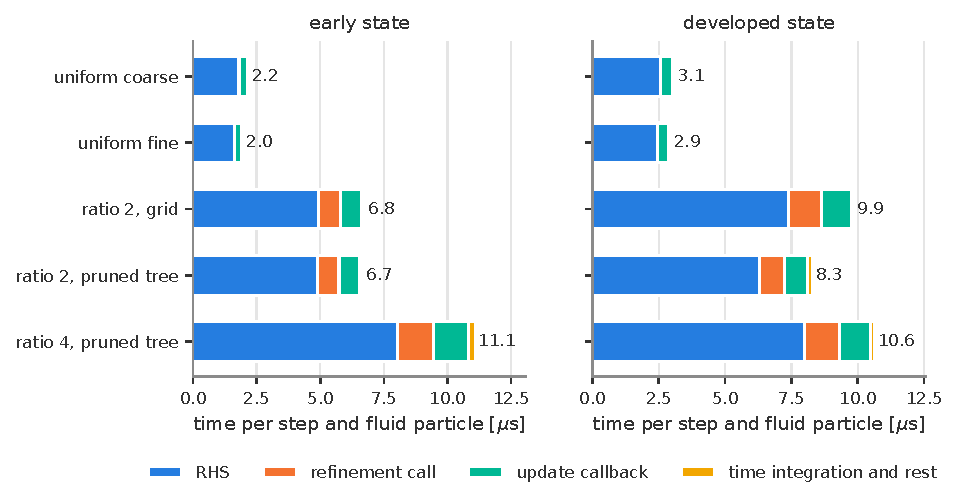
\includegraphics[width=\textwidth]{budget_per_particle}
  \caption{Time per step and fluid particle of the vortex street, uniform and refined, in
  the early and developed state. Before the load balancing of
  Section~\ref{sec:performance-measures}. \src{B1, B2}}
  \label{fig:performance-budget}
\end{figure}

\begin{table}[htb]
  \centering
  \caption{Shares of the step time [\%] of the refined vortex street. Before the load
  balancing. \src{B1}}
  \label{tab:performance-shares}
  \small
  \begin{tabular}{lrrrrrr}
\toprule
 & \multicolumn{2}{c}{ratio 2, grid} & \multicolumn{2}{c}{ratio 2, pruned tree} & \multicolumn{2}{c}{ratio 4, pruned tree} \\
\cmidrule(lr){2-3}\cmidrule(lr){4-5}\cmidrule(lr){6-7}
 & early & dev. & early & dev. & early & dev. \\
\midrule
step [ms] & 72 & 148 & 71 & 124 & 140 & 235 \\
fluid particles & 10.7k & 15.0k & 10.7k & 14.9k & 12.6k & 22.1k \\
\midrule
\textbf{RHS} & \textbf{72.8} & \textbf{74.9} & \textbf{73.5} & \textbf{75.9} & \textbf{72.4} & \textbf{75.3} \\
\quad interaction fluid-fluid & 27.1 & 30.3 & 21.7 & 25.1 & 19.5 & 24.2 \\
\quad interaction other pairs & 4.3 & 2.2 & 7.3 & 6.0 & 7.1 & 5.3 \\
\quad density (summation) & 13.7 & 15.3 & 16.4 & 16.6 & 18.3 & 18.2 \\
\quad average pressure and $\beta$ & 18.1 & 20.4 & 16.5 & 17.8 & 17.6 & 18.5 \\
\quad NHS update & 3.9 & 2.5 & 5.8 & 4.7 & 5.4 & 4.7 \\
\quad open boundary (characteristics) & 4.1 & 3.0 & 4.1 & 3.9 & 2.2 & 2.3 \\
\textbf{refinement call} & \textbf{13.1} & \textbf{12.7} & \textbf{12.4} & \textbf{11.4} & \textbf{13.0} & \textbf{12.2} \\
\quad shifting & 9.6 & 9.4 & 8.6 & 8.0 & 9.2 & 8.4 \\
\quad merge, split, criteria & 1.7 & 1.6 & 1.9 & 1.7 & 1.8 & 2.1 \\
\textbf{update callback} & \textbf{12.2} & \textbf{11.3} & \textbf{11.9} & \textbf{10.7} & \textbf{12.4} & \textbf{11.1} \\
\quad update of systems and NHS & 6.6 & 6.4 & 7.2 & 6.5 & 7.2 & 6.7 \\
\quad particle shifting (PST) & 4.3 & 4.4 & 3.5 & 3.3 & 3.9 & 3.4 \\
\textbf{time integration and rest} & \textbf{1.9} & \textbf{1.1} & \textbf{2.1} & \textbf{2.0} & \textbf{2.2} & \textbf{1.5} \\
\bottomrule
\end{tabular}

\end{table}

\begin{table}[htb]
  \centering
  \caption{Time per step and per fluid particle, uniform and refined (grid search for the
  uniform runs). Before the load balancing. \src{B1, B2}}
  \label{tab:performance-uniform}
  \small
  \begin{tabular}{lrrrrr}
\toprule
 & \multicolumn{2}{c}{uniform} & \multicolumn{3}{c}{refined} \\
\cmidrule(lr){2-3}\cmidrule(lr){4-6}
 & coarse & fine & r2 grid & r2 pruned & r4 pruned \\
\midrule
\multicolumn{6}{l}{\emph{early state}} \\
\quad fluid particles & 9.8k & 39.0k & 10.7k & 10.7k & 12.6k \\
\quad step [ms] & 21.4 & 76.8 & 72.1 & 71.1 & 139.5 \\
\quad step per fluid particle [$\mu$s] & 2.19 & 1.97 & 6.77 & 6.68 & 11.08 \\
\quad one RHS per fluid particle [$\mu$s] & 0.30 & 0.27 & 0.79 & 0.79 & 1.25 \\
\multicolumn{6}{l}{\emph{developed state}} \\
\quad fluid particles & 9.6k & 38.7k & 15.0k & 14.9k & 22.1k \\
\quad step [ms] & 29.7 & 113.9 & 147.6 & 123.9 & 234.9 \\
\quad step per fluid particle [$\mu$s] & 3.09 & 2.94 & 9.86 & 8.29 & 10.63 \\
\quad one RHS per fluid particle [$\mu$s] & 0.42 & 0.40 & 1.13 & 0.98 & 1.19 \\
\bottomrule
\end{tabular}

\end{table}

Three observations stand out.

\paragraph{The direct cost is small.}
The refinement call takes 11 to 13\,\% of the step, and about 70\,\% of it is the shifting
of the particles after splitting and merging (8 to 10\,\% of the step). Splitting, merging
and the evaluation of the criteria together take less than 2\,\%. The startup, which
refines the initial configuration until it is consistent with the criteria, takes 0.9\,s
at ratio~2 and 3.7\,s at ratio~4, about 80\,\% of it in the shifting. Compared to a wall
time of about 80\,s per unit of simulated time, it is negligible.
\src{B1}

\paragraph{The indirect cost dominates.}
Per fluid particle, a refined step costs 3.4 times as much as a uniform fine one in the
early state and 2.8 (pruned tree) to 3.4 times (grid) in the developed state. Most of
this is the RHS: one RHS evaluation costs 0.79\,$\mu$s per fluid particle at ratio~2,
compared to 0.27\,$\mu$s in the uniform fine simulation.

\paragraph{The shares hardly change.}
The distribution of the time over the parts of the step is nearly the same in both states,
at both ratios and with both searches: the RHS takes 72 to 76\,\%, the refinement call
11 to 13\,\%, the update callback 11 to 12\,\%. In the uniform simulations, the cost per
particle is the same at both spacings and grows by 40 to 50\,\% from the early to the
developed state. The growth with the developing flow is therefore not caused by the
refinement.

% ==========================================================================================
\section{Why a refined right-hand side is more expensive}
\label{sec:performance-rhs}

Figure~\ref{fig:performance-sections} compares the cost per fluid particle of the
individual loops with the uniform fine simulation. All loops over fluid neighbors (the
interaction, the summation density, the average pressure and $\beta$ of EDAC) cost 2.7 to
4.2 times as much per particle. The method of characteristics at the open boundaries costs
the same or less, since the open boundaries keep the coarse spacing. The pairs with the
walls and the cylinder are 4.1 times as expensive with the pruned tree: the cylinder pair
is still searched with the largest radius (Section~\ref{sec:performance-nhs}).

\begin{figure}[htb]
  \centering
  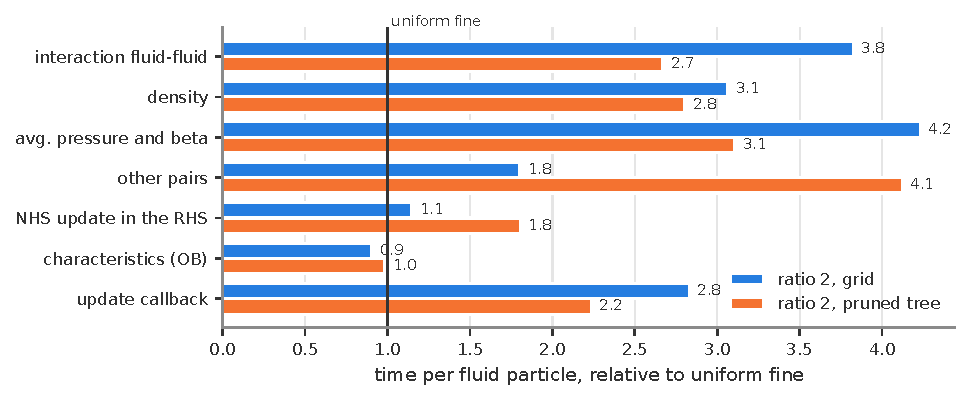
\includegraphics[width=\textwidth]{section_ratio}
  \caption{Time per fluid particle of the parts of a step at ratio~2, relative to the
  uniform fine simulation, developed state. Before the load balancing. \src{B1, B2}}
  \label{fig:performance-sections}
\end{figure}

To attribute the excess cost, the RHS of a single early state at ratio~2 was evaluated
with parts of the implementation changed one at a time: the particles dealt to the threads
in small blocks instead of contiguous chunks, refinement with a ratio of~1 (variable
smoothing lengths, but nothing refined), and the same number of particles in a uniform
simulation. Figure~\ref{fig:performance-decomposition} shows the result.

\begin{figure}[htb]
  \centering
  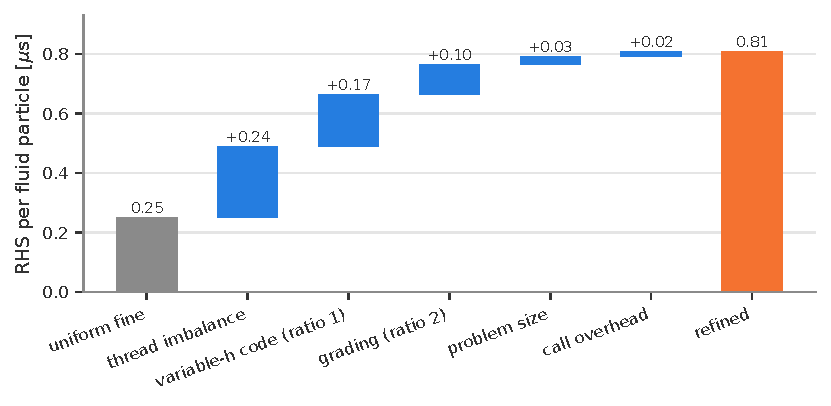
\includegraphics[width=\textwidth]{rhs_decomposition}
  \caption{Decomposition of the RHS cost per fluid particle, ratio~2, tree search, early
  state. Measured on an earlier commit, before the inlining fix and the load balancing of
  Section~\ref{sec:performance-measures}. \src{C1}}
  \label{fig:performance-decomposition}
\end{figure}

\paragraph{Thread imbalance (43\,\% of the excess).}
The loops over particles give each thread one contiguous share of equal size. New particles
from splitting are activated in the buffer at the end of the particle arrays, so the fine
particles, which have more neighbors in the tree search, are concentrated in the last
share. In the early state, 761 of the 1066 fine particles lie there, and the last thread
needs 2.8 times the mean time of a thread. The other threads wait for it. In the developed
state, with 47\,\% fine particles, the factor drops to 1.5. This cost is not inherent to
refinement but to the layout of the buffer, and Section~\ref{sec:performance-measures}
removes most of it.

\paragraph{Variable smoothing lengths (31\,\%).}
Already at a ratio of~1, where nothing is refined, the code for variable smoothing lengths
is more expensive: each pair evaluates the kernel gradient with both smoothing lengths, the
support is checked per pair, EDAC needs $\beta$, and the search uses one radius per
particle.

\paragraph{Grading (18\,\%).}
With two levels of particles, the search examines about twice as many candidates for the
same number of interacting neighbors, since most fluid particles lie in leaves of the tree
whose size follows the largest radius.

\paragraph{Problem size and call overhead (8\,\%).}
The rest is due to the different number of particles (cache effects) and the overhead
of the calls into the tree search.

% ==========================================================================================
\section{Implementation measures}
\label{sec:performance-measures}

Two changes to the implementation followed from the analysis. Neither changes the method.

\paragraph{Inlining.}
The loops that skip pairs outside of the support called the pair interaction through a
function that the compiler did not inline. Forcing the inlining reduced the RHS with the
grid search from 6.4 to 3.9\,ms at ratio~1 and from 10.2 to 7.6\,ms at ratio~2. Over whole
simulations, the step time decreased by about 23\,\% with the grid and 3\,\% with the tree
\src{I1}; the machine was loaded during this comparison, so the size of the gain is
uncertain, its direction is not. A single RHS gives bitwise identical results; over a whole simulation, a
difference in the last digit of one value appears after a few steps and changes some merge
decisions later. This sensitivity of the discrete refinement decisions to rounding is
inherent to the method; with a parallel update of the neighborhood search, it also makes two
runs of the same code differ.
\draftnote{the inline fix is in 92fef57, so it is included in all time budgets above;
the decomposition of Figure~\ref{fig:performance-decomposition} is from before it}

\paragraph{Load balancing.}
The neighbor loops of refined fluid systems now deal the active particles to the threads
in blocks of 64 particles in turn, instead of one contiguous share per thread. The order is
rebuilt whenever the set of active particles changes. Each particle still sums over its
neighbors in the same order, so the results are bitwise identical to the unbalanced
version over whole simulations. Figure~\ref{fig:performance-blocks} shows the effect of
the block size, Table~\ref{tab:performance-balancing} the comparison with the version
without balancing.

\begin{figure}[htb]
  \centering
  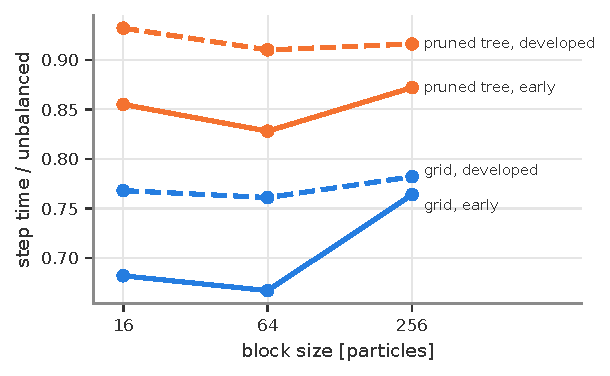
\includegraphics[width=0.62\textwidth]{block_size}
  \caption{Step time with load balancing relative to the unbalanced version, as a function
  of the block size, ratio~2. Median of six alternating repetitions in one process.
  \src{L1}}
  \label{fig:performance-blocks}
\end{figure}

\begin{table}[htb]
  \centering
  \caption{Effect of the load balancing (blocks of 64) on the step time, ratio~2.
  Early state: separate processes in alternating blocks, median and range over five blocks.
  Developed state: one process, median of six repetitions. \src{L1, L2}}
  \label{tab:performance-balancing}
  \small
  \begin{tabular}{lrr}
    \toprule
    & grid & pruned tree \\
    \midrule
    early, change of the step time & $-34.0\,\%$ ($-34.2$ to $-33.9$) &
      $-17.2\,\%$ ($-20.1$ to $-16.6$) \\
    early, A/A noise & 0.5\,\% & 4.4\,\% \\
    developed, step time [ms] & 146 $\to$ 111 ($-24\,\%$) & 114 $\to$ 104 ($-9\,\%$) \\
    \bottomrule
  \end{tabular}
\end{table}

Blocks of 64 particles were the best of the sizes tried in all four cases. The gain is
largest in the early state, where the imbalance is largest. With the balancing, one RHS of
the developed state costs about 0.8 to 0.9\,$\mu$s per fluid particle with the pruned tree,
which is 2.0 to 2.2 times the cost of the uniform fine simulation instead of 2.5 times.
\draftnote{estimate from two different scripts; measure the time budget with balancing}

% ==========================================================================================
\section{Choice of the neighborhood search}
\label{sec:performance-nhs}

With the grid search, every particle searches with the largest radius, which belongs to the
coarsest particles. The number of candidates per fine particle therefore grows with the
square of the spacing ratio in two dimensions, while the number of neighbors in its
support stays the same: within the largest radius, a fluid particle has 81 fluid
candidates at ratio~4 and 308 at ratio~8, of which 27 and 28 are in its support \src{N1}.
The tree search with per-particle radii avoids most of these candidates.

At ratio~2 the difference is small. Before the load balancing, the grid and the pruned tree
had the same step time in the early state (72 and 71\,ms), and the pruned tree was faster in
the developed state (124 and 148\,ms) \src{B1}. With the load balancing, the grid is faster
in the early state (47 and 56\,ms), and the pruned tree remains faster in the developed state
(104 and 111\,ms) \src{L1}. At higher ratios, the tree wins clearly
(Table~\ref{tab:performance-ratio}), and pruning adds a large part of the gain.

\begin{table}[htb]
  \centering
  \caption{Tree search compared to the grid search at higher spacing ratios, early state.
  Before the load balancing. The tree and the grid take slightly different time steps,
  so the comparison uses the wall time per unit of simulated time. \src{N1}}
  \label{tab:performance-ratio}
  \small
  \begin{tabular}{lrr}
    \toprule
    & ratio 4 & ratio 8 \\
    \midrule
    step time grid / tree / pruned tree [ms] & 214 / 196 / 153 & 666 / 486 / 385 \\
    wall time per simulated time, tree / pruned tree vs.\ grid &
      $-12\,\%$ / $-30\,\%$ & $-30\,\%$ / $-44\,\%$ \\
    refinement call, tree / pruned tree vs.\ grid & $-16\,\%$ / $-35\,\%$ &
      $-36\,\%$ / $-49\,\%$ \\
    \bottomrule
  \end{tabular}
  \draftnote{ratio 4: only 1 of 8 blocks without disturbance; repeat on a quiet machine}
\end{table}

One pair still uses the largest radius with either search: the fluid and the cylinder. The
per-particle radii are only used when both systems have variable smoothing lengths, and the
cylinder has a constant one. At ratio~8, each fluid particle examines 109 cylinder
particles, of which 0.3 are in its support on average; this pair takes 5.5 of the 13.7\,ms
of the interaction with the pruned tree \src{N1}. A query radius per particle for wall
systems would remove this cost.

% ==========================================================================================
\section{Discussion}
\label{sec:performance-discussion}

The refinement call itself is cheap. The cost of the refinement lies in the more expensive
right-hand side, which at ratio~2 costs two to three times as much per particle as in a
uniform simulation. About half of this excess was an imbalance of the threads caused by the
layout of the particle buffer, which the load balancing removes without changing the
results. What remains is mostly the code for variable smoothing lengths and the search over
a graded particle distribution.

In the vortex street at ratio~2, the refined simulation has 2.6 times fewer fluid particles
than the uniform fine one in the developed state, and a step costs about 2.5 to 2.8 times as
much per particle. The two effects nearly cancel: the refined simulation needs about
110 to 120\,s per unit of simulated time, the uniform fine one 106\,s \src{B1, B2, L1}. A
refined simulation is therefore not faster than a uniform simulation at its finest spacing
in this case. Whether it reaches a given accuracy faster than a uniform simulation at an
intermediate spacing is examined in Chapter~\ref{ch:vortex-street}.
\draftnote{the particle saving grows with the ratio and with the size of the domain
relative to the refined region; the cost per particle grows less from ratio~2 to~4
(1.0 to 1.2\,$\mu$s per RHS, developed) -- worth one sentence once measured with balancing}

\paragraph{Limitations.}
The measurements cover one test case at one resolution, on 8 threads of one CPU. Scaling to
more threads, larger problems and GPUs was not measured. The numbers in this chapter come
from several versions of the code during the development \draftnote{remove after the
stage 2 measurements}.

\paragraph{Possible improvements.}
The following were identified but not implemented, since they concern the general code or
the neighborhood search rather than the refinement:
\begin{itemize}
  \item The summation density and the average pressure with $\beta$ search the same fluid
        neighbors in separate loops. One combined loop is estimated to save 7 to 10\,\% of
        the step, in uniform simulations as well.
  \item With an integrator whose last stage is evaluated at the end of the step, the update
        callback recomputes the state that the last RHS evaluation has already prepared
        (6 to 7\,\% of the step).
  \item The tree search could prune more aggressively and refine its leaves for graded
        distributions, and walls could use per-particle query radii.
\end{itemize}

\end{document}
